\chapter{Implementation of the Info-Terminal}
The info-terminal has been created by using a \ac{wp} plugin called SmartSlider3\footnote{https://wordpress.org/plugins/smart-slider-3/}. SmartSlider3 is a free plugin available in the WordPress plugin repository. It enables the creation and designation of slider easily with a lot of features.

\section{Getting Started}
First, the SmartSlider3 plugin has to be added and activated in the WordPress. After the activation, the left menu list will receive a new entry 'Smart Slider'. Click it will bring the Smart Slider dashboard interface, where slider can created, modified and deleted. A new slider can be created by clicking the 'New Slider' tile on the dashboard. Here the following details have been given:
\begin{itemize*}
\item Slide name: Info Terminal
\item Width: 1920 px
\item Height: 1080 px
\item Preset: Default
\item Import Sample Sliders: none
\end{itemize*}
\begin{figure}[ht]
\caption{Creating a new slider}
\label{creating-a-new-slider}
\centering
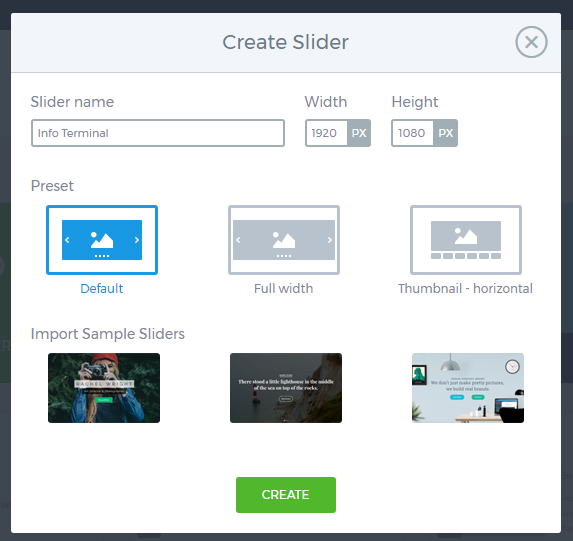
\includegraphics[height=4cm,keepaspectratio]{info-terminal/creating-new-slider.png}
\end{figure}

After the above mentioned details have been given, the creation of new slider have been proceed by clicking the 'Create' button.

\section{Slider Settings}
There are a few general settings that has to be configured after creating a new slider. The slider settings options can be found immediately after getting into the 'Info Terminal' slider.

subsection*{General Settings}
Under 'General' tab, two settings has be changed, which are:
\begin{itemize*}
\item Align: Center
\item Main animation properties (Duration): 600 ms
\end{itemize*}

\subsection*{Size Settings}
Here, the following attributes has to be changed:
\begin{itemize*}
\item Slide size (Width): 1920 px
\item Slide size (Height): 968 px
\item Slider height (Min): 300 px
\item Slider height (Max): 968 px
\item Slider width (max): 1920 px
\end{itemize*}

\subsection*{Autoplay Settings}
Here, the following attributes has to be changed:
\begin{itemize*}
\item Autoplay (Enabled): True
\item Autoplay (Interval): 5000 ms
\end{itemize*}

\subsection*{Arrow Settings}
Here, the following attributes has to be set:
\begin{itemize*}
\item Previous (Color): 999999FF
\item Style: Static
\end{itemize*}

\subsection*{Autoplay Icon Settings}
By default, the autoplay mode in the slider is turned off. This mode has to be turned on as shown in Figure~\ref{autoplay-icon-on} and the rest the of settings are left to default settings.
\begin{figure}[ht]
\caption{Autoplay Icon Settings}
\label{autoplay-icon-on}
\centering
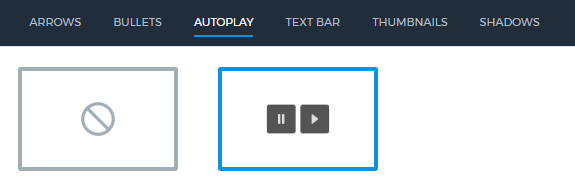
\includegraphics[height=3cm,keepaspectratio]{info-terminal/autoplay-icon-on.png}
\end{figure}

\subsection*{Thumbnails Setting}
After enabling the Thumbnails, which by default is turned off, the following attributes have to be set.
\begin{itemize*}
\item Thumbnail size (Width): 150 px
\item Thumbnail size (Height): 100 px
\item Position: Outer, bottom
\end{itemize*}

\subsection*{Publish Setting}
Under the 'Publish' tab, the shortcode of the created slider has to be taken note (refer Figure~\ref{slider-shortcode}). In this case, the short code is \texttt{\[smartslider3 slider=1\]}. This code will be used to insert the slider into the WordPress web page as discussed in the Section~\ref{inserting-slider-into-web-page}.

\section{Inserting Slider Into Web Page} \label{inserting-slider-into-web-page}
A new WordPress page has to be created through the  \scalerel*{
\includegraphics{info-terminal/add-new-page.png}}{B} option under the \scalerel*{
\includegraphics{info-terminal/pages-menu.png}}{B} menu.
\begin{enumerate}
\item The title of page has been given as 'Info Terminal' in the 'Title' field.
\item The permalink or slug has been set to \texttt{info/}.
\item The shortcode, which have been noted down from previous section has to be pasted or typed in the editor.
\item Lastly, the template of this web page has been changed from 'Default Template' to 'Blank Slate'.
\end{enumerate}

\section{Creating and Setting Slide}
After setting the slider setting, slide can be created and set. The slider can be created by clicking the 'NEW SLIDE' green icon tile as shown in the Figure~\ref{new-slide-tile-icon}. After clicking it, we will be prompted to select an image. Here, any dummy image has to be chosen for time being until the slide background is set in the next step.
\begin{figure}[ht]
\caption{New slide tile icon}
\label{new-slide-tile-icon}
\centering

\includegraphics[height=2cm,keepaspectratio]{info-terminal/new-slide-tile-icon.png}
\end{figure}

Next, after the slide has been created, the following Background and Settings has to be given as shown in the Figure~\ref{slide-general-settings}. Through the 'Background' tab as shown in the Figure~\ref{slide-background}, these attributes has to be set to the following:
\begin{itemize*}
\item Background: Color
\item Color: FAFAFAFF
\end{itemize*}
Where else, through the 'Settings' tab, the name of the current slide along with the respective thumbnail can be inserted.
\begin{figure}[ht]
\caption{Slide settings}
\label{slide-general-settings}
\centering
	\begin{subfigure}{.49\linewidth}
	\caption{Slide background}
	\label{slide-background}
	\centering
	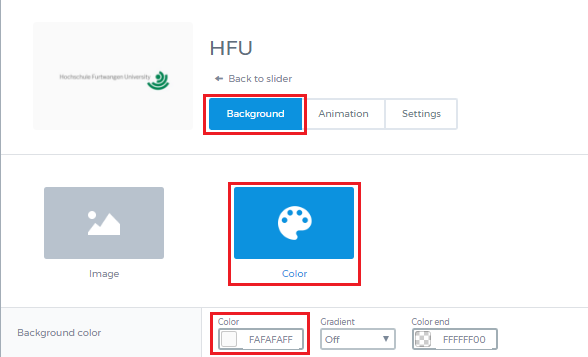
\includegraphics[height=3cm,keepaspectratio]{info-terminal/slide-background.png}
	\end{subfigure}
	\begin{subfigure}{.49\linewidth}
	\caption{Slide's name and thumbnail}
	\label{slide-settings}
	\centering
	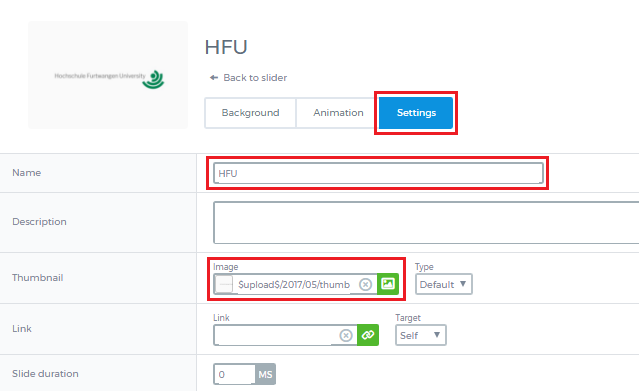
\includegraphics[height=3cm,keepaspectratio]{info-terminal/slide-settings.png}
	\end{subfigure}
\end{figure}

\section{Adding Home Button}
Home button has been added to all slides manually. The following steps explain how it is done in detail. First the 'Text layer' has to be added to the slide by clicking the \scalerel*{
\includegraphics{info-terminal/text-layer-icon.png}}{B} icon that can be found to the right of the slide view. This will bring up a widget (refer Figure~\ref{text-layer-widget}, where the following has to be set.
\begin{figure}[ht]
\caption{Text layer widget}
\label{text-layer-widget}
\centering
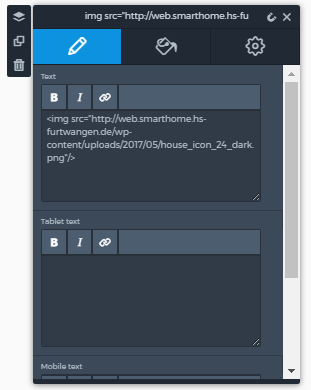
\includegraphics[height=3cm,keepaspectratio]{info-terminal/text-layer-widget.png}
\end{figure}

Through the first tab with icon \scalerel*{
\includegraphics{info-terminal/pencil-icon.png}}{B} in the 'Text' field, the following HTML codes has to be entered:
\begin{lstlisting}
<img src="http://web.smarthome.hs-furtwangen.de/wp-content/
      uploads/2017/05/house_icon_24_dark.png"/>
\end{lstlisting}

Through the third tab with icon \scalerel*{
\includegraphics{info-terminal/widget-gear-icon.png}}{B}, following has to be set:
\begin{itemize*}
\item Align: \scalerel*{
\includegraphics{info-terminal/home-button-align.png}}{B}
\item Position X: 25 px
\item Position Y: 25 px
\item Width: Auto
\item CSS class: home-button cursor-pointer
\end{itemize*}

Next, through the \scalerel*{
\includegraphics{info-terminal/pages-menu.png}}{B} menu, 'Edit' option has to clicked to open the 'Info Terminal' page, which has been created in the Section~\ref{inserting-slider-into-web-page}.

Under the 'Scripts n Styles' section, the following CSS codes has to be added under the 'Styles' tab:
\begin{lstlisting}
.cursor-pointer {
	cursor: pointer;
	text-decoration: none;
}
\end{lstlisting}

After that, under the 'Scripts' tab, the following \ac{js} codes has been added:
\begin{lstlisting}
window.n2ss.ready(1, function(slider){
	jQuery('.home-button').click(function(){
		window.location.href="/";
	});
});
\end{lstlisting}

These JavaScript codes give the callback functionality to the home button found on every slides. When, it is clicked, the browser takes the user to the website's home page.

\section{Adding Header} \label{sec:adding-header}
Header elements can be added into the slide by clicking on \scalerel*{
\includegraphics{info-terminal/header-icon.png}}{B} icon which can be found on the left side of the slide view. This will bring up a widget where the header text can be entered as shown in Figure~\ref{fig:info-terminal-adding-header-text}. By click the \scalerel*{
\includegraphics{info-terminal/widget-gear-icon.png}}{B} on the widget, the alignment, position and size (width, height) of the header element can be set, shown in Figure~\ref{fig:info-terminal-header-settings}.

\begin{figure}[ht]
	\begin{subfigure}{.49\textwidth}
	\caption{Adding header}
	\label{fig:info-terminal-adding-header-text}
	\centering
	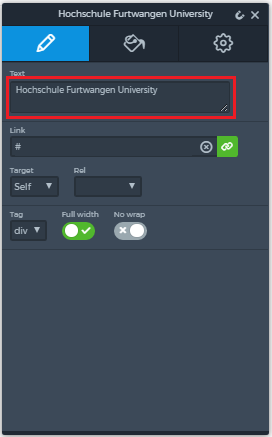
\includegraphics[height=3.5cm,keepaspectratio]{info-terminal/adding-header-element.png}
	\end{subfigure}
	\begin{subfigure}{.49\textwidth}
	\caption{Header element settings}
	\label{fig:info-terminal-header-settings}
	\centering
	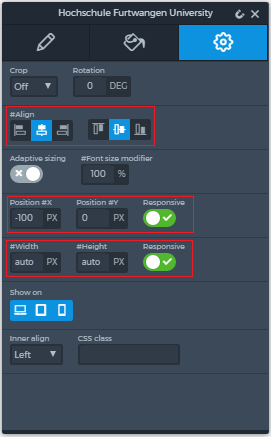
\includegraphics[height=3.5cm, keepaspectratio]{info-terminal/header-settings.png}
	\end{subfigure}
\end{figure}

\section{Adding Images}
Images can be added to slide by clicking the \scalerel*{
\includegraphics{info-terminal/image-icon.png}}{B} icon on left of the slide viewer. Clicking this icon will bring up the media selector window where an image has to be selected. After an image had been selected, the image widget can be seen with the selected image as shown in Figure~\ref{fig:image-widget}. Here also the gear icon can be selected to apply futher settings to the image such as positioning, alignment and sizing.

\begin{figure}[ht]
\caption{Image widget}
\label{fig:image-widget}
\centering
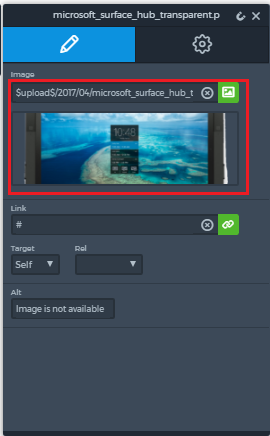
\includegraphics[height=3.5cm,keepaspectratio]{info-terminal/added-image.png}
\end{figure}

\section{Creating Overview Buttons}
Each spaces such as (living room, kitchen, washroom, workspace and multimedia room) will be presented with overview buttons as shown in Figure~\ref{fig:oveview-buttons}. This section will explain on how to create an overview button.

\begin{figure}[ht]
\caption{Overview buttons}
\label{fig:overview-button}
\centering
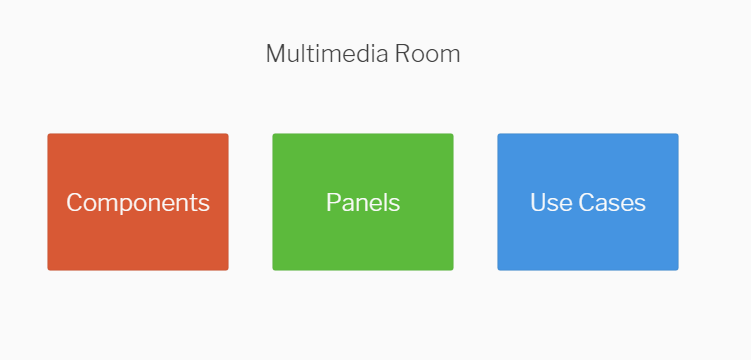
\includegraphics[height=3.5cm,keepaspectratio]{info-terminal/overview-buttons.png}
\end{figure}

\subsection*{Step 1: Adding Header Element}
An header element has to be added to slide as discussed in the Section~\ref{sec:adding-header}. Here the text should be given either 'Components', 'Panels' or 'Use Cases'. 

\subsection*{Step 2: Header Designing}
After adding a appropriate text, the header element has to be designed clicking the \scalerel*{
\includegraphics{info-terminal/widget-paint-icon.png}}{B}. Clicking this, will show the CSS designing panel as shown in the Figure~\ref{fig:header-designing}. Here, the following design settings have to changed:
\begin{itemize*}
\item Color: FAFAFAFF
\item Line height: 5.75
\item Text align: \scalerel*{
\includegraphics{info-terminal/align-center.png}}{B}
\item Background color: D85935FF (eg. for 'Components' button)
\item Border: 1 px Solid BB4A28FF (eg. for 'Components' button)
\item Border radius: 5 px
\end{itemize*}

\begin{figure}[ht]
\caption{Designing header element}
\label{fig:header-designing}
\centering
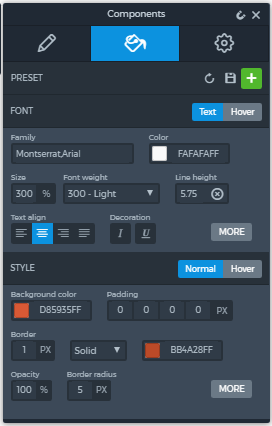
\includegraphics[height=3.5cm,keepaspectratio]{info-terminal/header-designing.png}
\end{figure}

subsection*{Step 3: Header Settings}
Next, the header element need to be set. The setting screen can be opened by clicking the \scalerel*{
\includegraphics{info-terminal/widget-gear-icon.png}}{B}. Here besides alignment, positioning and sizing, the CSS class has to be set, which is important. In the CSS class text field as shown in Figure~\ref{fig:css-class-field}, the following text has to be entered:
\begin{lstlisting}
card-4 living-room-components
\end{lstlisting}

The \texttt{card-4} is constant for all overview button. The \texttt{living-room-} is depends on for which space the button are being added. For an example, for \emph{kitchen}, this part has to be replaced with \texttt{kitchen-}. The last part of is \texttt{components}. This part has to replaced accordingly. For an example, for \emph{panels}, this part should be replaced with \texttt{panels} and for \emph{use cases} with \texttt{use-cases}.

\begin{figure}[ht]
\caption{Adding CSS Class}
\label{fig:css-class-field}
\centering
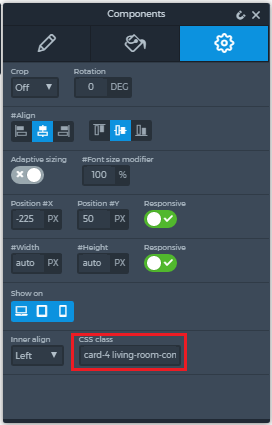
\includegraphics[height=3.5cm,keepaspectratio]{info-terminal/css-class-field.png}
\end{figure}

Next by toggling to \emph{Hover} section by clicking \scalerel*{
\includegraphics{info-terminal/design-hover.png}}{B} icon, the following entries have to be given:
\begin{itemize*}
\item Background color: BB4A28FF
\item Padding: 0 0 0 0 px
\item Border: 1 px Solid BB4A28FF
\item Border radius: 5 px
\end{itemize*}

\subsection*{Step 3: Adding CSS}
Next, click the \scalerel*{
\includegraphics{info-terminal/pages-menu.png}}{B}. Then edit the 'Info-Terminal' page. Under the 'Style' tab in the 'Scripts n Styles' section, few lines of CSS codes have to be added for additional designing of the overview button as listed below:
\begin{lstlisting}
.card-4 {
	min-width: 19\%;
	min-height: 30\%;
	border-radius: 5px;
	box-shadow: 0 14px 28px rgba(0,0,0,0.25), 0 10px 10px rgba(0,0,0,0.22);
	cursor: pointer;
}

.card-4 div {
	position: absolute;
	min-width: 100\%;
	min-height: 100\%;
}
\end{lstlisting}

\subsection*{Step 4: Adding JavaScript Callback}
Lastly, a JavaScript callback has to be added to button, so that when the button is clicked, the slider takes the user to to respective slide. This can be done by adding the following code under the \emph{Script} tab under the \emph{Scripts n Styles} section.

\begin{lstlisting}
window.n2ss.ready(1, function(slider){
	jQuery('.living-room-components').click(function() {
		slider.slide(10);
	});
});
\end{lstlisting}

Above is an example of JavaScript callback implemented by using jQuery \texttt{.click} function. Here, the \texttt{'.living-room-components'} is the text entered in the CSS Class text field as discussed in the Step 3. The line \texttt{slider.slide(10)} is the execution telling the slider to move to slide number 10. Here, the destination slide is at index 10 starting with the first slide at index 0.

\section{Creating Component Buttons}
This section will discuss how to create the component buttons as shown in the Figure~\ref{fig:component-buttons}. The component buttons shown in figure belongs to the one that can be found in the living room. In this case, there are only two components in the living room, namely \emph{Surface Hub} and \emph{BenQ Smart Projector}. In order to create this buttons, there are few steps to be taken which will be discussed here.

\subsection*{Step 1: Adding header element}
Header element can be added to the slider by clicking the \scalerel*{
\includegraphics{info-terminal/header-icon.png}}{B}. Then, the corresponding text has to be added to the \emph{Text} field which can be found on the widget first tab.

\subsection*{Step 2: Designing the header element}
Next, the header element has to be designed. To proceed with designing, click on the \scalerel*{
\includegraphics{info-terminal/widget-paint-icon.png}}{B}. In this section of the widget as shown in the Figure~\ref{fig:component-button-designing}, following entries have to be changed:
\begin{itemize*}
\item Color: 414141FF
\item Line height: 1.5
\item Background color: CED3D5FF
\item Padding: 5 0 5 0 px
\item Border: 1 px solid 81898DFF
\item Border radius: 5px
\end{itemize*}

Next by toggling to \emph{Hover} section by clicking \scalerel*{
\includegraphics{info-terminal/design-hover.png}}{B} icon, the following entries have to be given:
\begin{itemize*}
\item Background color: BDC1C3FF
\item Padding: 5 0 5 0 px
\item Border: 1 px Solid 81898DFF
\item Border radius: 5 px
\end{itemize*}

\begin{figure}[ht]
\caption{Designing component buttons}
\label{fig:component-button-designing}
\centering
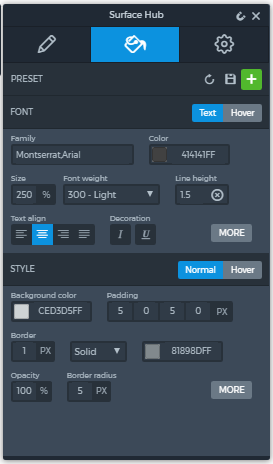
\includegraphics[height=3.5cm,keepaspectratio]{info-terminal/component-button-designing.png}
\end{figure}

\subsection*{Step 3: Setting Header Element}
The header element has to be set with following settings. The setting panel of the header element can be opened by clicking the \scalerel*{
\includegraphics{info-terminal/widget-gear-icon.png}}{B}. Here, the following entries has to be set:
\begin{itemize*}
\item Align:
\item Width: 1000 px
\item Height: auto
\item CSS claa: card-1 components-surface-hub
\end{itemize*}

CSS Class with text \texttt{card-1 components-surface-hub} is very important. The \texttt{card-1} is the reference to CSS styling which will be discussed in the next section. Whereby \texttt{components-surface-hub} is the reference for the JavaScript callback function. In this case, it refers to the destination slide which contains the component Surface Hub.

\subsection*{Adding CSS Styling}
To add the CSS styling for the component buttons, navigate to \scalerel*{
\includegraphics{info-terminal/pages-menu.png}}{B}. Edit the \emph{Info Terminal}. Under the \emph{Styles} tab under \emph{Scripts n Styles} section, the following CSS codes have to be added:

\begin{lstlisting}
.card-1 {
	border-radius: 5px;
	box-shadow: 0 5px 10px rgba(0,0,0,0.19), 0 6px 6px rgba(0,0,0,0.23);
	cursor: pointer;
}
\end{lstlisting}

\subsection*{Adding JavaScript Callback}
The JavaScript callback is a small codes that will get executed when the user click on the component buttons. This codes will be added to the \emph{Scripts} tab under the \emph{Scripts n Styles} section. Here, the following codes have to be added:

\begin{lstlisting}
window.n2ss.ready(1, function(slider){
	jQuery('.components-surface-hub').click(function(){
		slider.slide(11);
	});
});
\end{lstlisting}

The example callback function above contains the reference \path{'.components-surface-hub'}. When the button with this reference get clicked, the \texttt{.click()} function will be executed which will slide the slider to to slide with index 10. The slide number 10 should contain, in this case, the \emph{Surface Hub}. The index counting starts from 0.

\section{Creating Panel Buttons}
This section will explain on how to create a panel button as shown in the Figure~\ref{fig:panel-buttons}. Panel buttons are buttons that have been used as navigation to items that can be found on the panels in the lab. These buttons have been created with images of item itself.

\begin{figure}[ht]
\caption{Panel buttons}
\label{fig:panel-buttons}
\centering
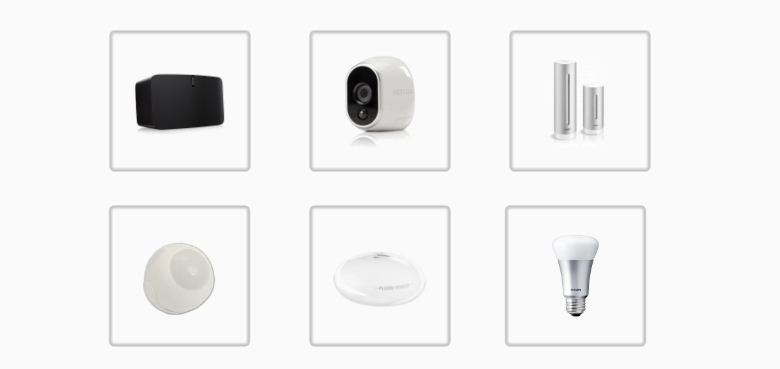
\includegraphics[height=3.5cm,keepaspectratio]{info-terminal/panel-buttons.png}
\end{figure}

\subsection*{Step 1: Adding Text Layer}
In order to add or create a panel button, a text layer has to be added by clicking \scalerel*{
\includegraphics{info-terminal/text-layer-icon.png}}{B} icon that can be found on left of the slide viewer. This is bring up the text layer widget as shown in the Figure~\ref{fig:text-layer-widget}. In the \emph{Text} field which can be found under \scalerel*{
\includegraphics{info-terminal/pencil-icon.png}}{B}, the following HTML codes have to be added. This code will result in the following button containing the Sonos Play:5 speaker as the button image.

\begin{lstlisting}
<div class="panel-nav-container panels-sonos-play5">
	<span class="span-helper"></span>
	<img src="/wp-content/uploads/2017/04/play5-blk-angle.png" alt="Sonos Play:5" style="vertical-align:middle;max-width:75%;max-height:75%;">
</div>
\end{lstlisting}

\subsection*{Step 2: Setting of Text Layer}
Setting of the text layer can be accessed by clicking the \scalerel*{
\includegraphics{info-terminal/widget-gear-icon.png}}{B}. Here, only two settings has to be changed as listed below:
\begin{itemize*}
\item Width: 200 px
\item Height: 200 px
\end{itemize*}

Apart from the width and height, the positioning of the button in X and Y direction has to be set accordingly as can be seen in Figure~\ref{fig:panel-buttons}.

\subsection*{Step 3: Adding CSS Styling}
To style the button, CSS styling has to applied. Edit the \emph{Info Terminal} page which can be found under \scalerel*{
\includegraphics{info-terminal/pages-menu.png}}{B}. Under the \emph{Styles} tab under \emph{Scripts n Styles} section, the following CSS code has to be added:
\begin{lstlisting}
.panel-nav-container {
	background-color: #fff;
	text-align: center;
	width: 100%;
	height: 100%;
	border-radius: 10px;
	border: 1px solid #aaa;
	box-shadow: 0 0 5px 2px rgba(0, 0, 0, 0.2) inset;
	cursor: pointer;
	position: absolute;
}

.panel-nav-container:hover {
	border: 1px solid #008855;
	box-shadow: 0 0 5px 2px rgba(0, 136, 85, 0.2) inset;
}

.span-helper {
	display: inline-block;
	height: 100%;
	vertical-align: middle;
}

.panel-nav-container img {
	transform: scale(1);
	transition: transform 0.5s;
	transition-timing-function: ease;
}

.panel-nav-container:hover img {
	transform: scale(1.1);
}
\end{lstlisting}

This CSS code will style the panel button and the image of button as well. The CSS with \emph{:hover} tags add the hover effect to buttons.

\subsection*{Step 4: Adding JavaScript Callback}
Lastly, the JavaScript callback function has to be added to the button when the user click on the buttons. The JavaScript callback has to be added under the \emph{Scripts} tab under the \emph{Scripts n Styles} section of the \emph{Info Terminal} page.
\begin{lstlisting}
window.n2ss.ready(1, function(slider){
	jQuery('.panels-sonos-play5-2').click(function(){
		slider.slide(55);
	});
});
\end{lstlisting}

\section{Creating Use-Cases Buttons}
Use-cases buttons are the buttons used to navigate user to the use-cases that can be found in the lab. A use-case button contains an image and a short descriptive text below the text as shown in Figure~\ref{fig:use-cases-buttons}

\begin{figure}[ht]
\caption{Use-cases buttons}
\label{fig:use-cases-buttons}
\centering
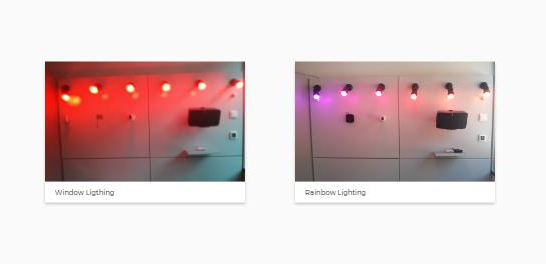
\includegraphics[height=3.5cm,keepaspectratio]{info-terminal/use-cases-buttons.png}
\end{figure}

\subsection*{Step 1: Adding Text Layer}
Begin by adding the text layer to the slide by clicking the \scalerel*{
\includegraphics{info-terminal/text-layer-icon.png}}{B}. In the \emph{Text} field under the \scalerel*{
\includegraphics{info-terminal/pencil-icon.png}}{B} the following HTML codes have to be entered:

\begin{lstlisting}
<img src="/wp-content/uploads/2017/05/window-light-on.jpg" alt="Window Lighting" style="width:400px;">
<div class="use-cases-desc">
	<p>Window Ligthing</p>
</div>
\end{lstlisting}

The above code is an example of use-cases button for \emph{Window Lighting}.

\subsection*{Step 2: Adding CSS Class}
After adding the HTML codes to the \emph{Text} field, class text has to be added to the \emph{CSS class} field which can be found under the  \scalerel*{
\includegraphics{info-terminal/widget-gear-icon.png}}{B}. Here the following CSS class has to be entered:
\begin{lstlisting}
use-cases-container use-cases-window-ligthing
\end{lstlisting}

The \texttt{use-cases-container} will be used as a reference for CSS styling. And the \texttt{use-cases-window-lighting}, in this case as an example for window lighting use-cases button, will be used as CSS class reference for the JavaScript callback.

\subsection*{Step 3: Adding CSS Styling}
The use-cases buttons have been styled by using custom CSS code. The CSS code has been entered under the \emph{Styles} tab under the \emph{Scripts n Styles} section of the \emph{Info Terminal} page. The following CSS code has been added for styling:
\begin{lstlisting}
div.use-cases-container {
	max-width: 20%;
	background-color: white;
	box-shadow: 0 4px 8px 0 rgba(0, 0, 0, 0.2);
	cursor: pointer;
	transition: box-shadow 0.5s;
	transition-timing-function: ease;
}

div.use-cases-desc {
	border-top: 1px solid #aaa;
	text-align: center;
	padding: 3.5% 5.5%;
}

div.use-cases-container:hover {
	box-shadow: 0 10px 20px 5px rgba(0, 0, 0, 0.2);
}
\end{lstlisting}

\subsection*{Step 4: Adding JavaScript Callback}
Lastly, JavaScript callback has to be programmed so that the slider will navigate to the destination slide when the user click on the use-cases buttons. The JavaScript callback script has to be added under the \emph{Scripts} tab under the \emph{Scripts n Styles}.

\begin{lstlisting}
window.n2ss.ready(1, function(slider){
	jQuery('.use-cases-window-ligthing').click(function(){
		slider.slide(62);
	});
	jQuery('.use-cases-rainbow-ligthing').click(function(){
		slider.slide(63);
	});
});
\end{lstlisting}

\section{Creating Breadcrumb}
Breadcrumb, as shown in the Figure~\ref{fig:breadcrumb}, is the navigation bar that can be found on the slides, where user can navigate from the current level to the upper hierarchy level.

\begin{figure}[ht]
\caption{Breadcrumb}
\label{fig:breadcrumb}
\centering
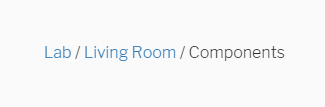
\includegraphics[height=2.5cm,keepaspectratio]{info-terminal/breadcrumb.png}
\end{figure}

\subsection*{Step 1: Adding Text Layer}
Start creating a breadcrumb by adding a text layer to the slide by clicking \scalerel*{
\includegraphics{info-terminal/text-layer-icon.png}}{B} icon

\begin{lstlisting}
<span class="breadcrumb_link breadcrumb-lab">Lab</span> / <span class="breadcrumb_link lab-multimedia-room">Multimedia Room</span> / Use Cases
\end{lstlisting}

\subsection*{Step 2: Adding CSS Styling}
Next, CSS styling has to be applied. The CSS code has to entered unde the \emph{Styles} tab under the \emph{Scripts n Styles} section in the Info Terminal page.

\begin{lstlisting}
.breadcrumb_link {
	color: #337ab7;
	cursor: pointer;
}

.breadcrumb_link:hover {
	filter: brightness(70%);
	text-decoration: underline;
}
\end{lstlisting}

\subsection*{Step 3: Adding JavaScript Callback}
Lastly, JavaScript callback script has to be added so that when the user click on the breadcrumb link, the slider will take user to the destination slide.
\begin{lstlisting}
window.n2ss.ready(1, function(slider){
	jQuery('.breadcrumb-lab').click(function(){
		slider.slide(4);
	});
});
\end{lstlisting}